\documentclass[journal, a4paper]{IEEEtran}

% some very useful LaTeX packages include:
\usepackage{multirow}
\usepackage{graphicx}
\usepackage[table]{xcolor} % for rowcolor
\usepackage{framed}
\usepackage{booktabs}   % for medrule and toprule
\usepackage{import}     % to import tables
%\usepackage{cite}      % Written by Donald Arseneau
                        % V1.6 and later of IEEEtran pre-defines the format
                        % of the cite.sty package \cite{} output to follow
                        % that of IEEE. Loading the cite package will
                        % result in citation numbers being automatically
                        % sorted and properly "ranged". i.e.,
                        % [1], [9], [2], [7], [5], [6]
                        % (without using cite.sty)
                        % will become:
                        % [1], [2], [5]--[7], [9] (using cite.sty)
                        % cite.sty's \cite will automatically add leading
                        % space, if needed. Use cite.sty's noadjust option
                        % (cite.sty V3.8 and later) if you want to turn this
                        % off. cite.sty is already installed on most LaTeX
                        % systems. The latest version can be obtained at:
                        % http://www.ctan.org/tex-archive/macros/latex/contrib/supported/cite/

\usepackage{graphicx}   % Written by David Carlisle and Sebastian Rahtz
                        % Required if you want graphics, photos, etc.
                        % graphicx.sty is already installed on most LaTeX
                        % systems. The latest version and documentation can
                        % be obtained at:
                        % http://www.ctan.org/tex-archive/macros/latex/required/graphics/
                        % Another good source of documentation is "Using
                        % Imported Graphics in LaTeX2e" by Keith Reckdahl
                        % which can be found as esplatex.ps and epslatex.pdf
                        % at: http://www.ctan.org/tex-archive/info/

%\usepackage{psfrag}    % Written by Craig Barratt, Michael C. Grant,
                        % and David Carlisle
                        % This package allows you to substitute LaTeX
                        % commands for text in imported EPS graphic files.
                        % In this way, LaTeX symbols can be placed into
                        % graphics that have been generated by other
                        % applications. You must use latex->dvips->ps2pdf
                        % workflow (not direct pdf output from pdflatex) if
                        % you wish to use this capability because it works
                        % via some PostScript tricks. Alternatively, the
                        % graphics could be processed as separate files via
                        % psfrag and dvips, then converted to PDF for
                        % inclusion in the main file which uses pdflatex.
                        % Docs are in "The PSfrag System" by Michael C. Grant
                        % and David Carlisle. There is also some information
                        % about using psfrag in "Using Imported Graphics in
                        % LaTeX2e" by Keith Reckdahl which documents the
                        % graphicx package (see above). The psfrag package
                        % and documentation can be obtained at:
                        % http://www.ctan.org/tex-archive/macros/latex/contrib/supported/psfrag/

%\usepackage{subfigure} % Written by Steven Douglas Cochran
                        % This package makes it easy to put subfigures
                        % in your figures. i.e., "figure 1a and 1b"
                        % Docs are in "Using Imported Graphics in LaTeX2e"
                        % by Keith Reckdahl which also documents the graphicx
                        % package (see above). subfigure.sty is already
                        % installed on most LaTeX systems. The latest version
                        % and documentation can be obtained at:
                        % http://www.ctan.org/tex-archive/macros/latex/contrib/supported/subfigure/

\usepackage{url}        % Written by Donald Arseneau
                        % Provides better support for handling and breaking
                        % URLs. url.sty is already installed on most LaTeX
                        % systems. The latest version can be obtained at:
                        % http://www.ctan.org/tex-archive/macros/latex/contrib/other/misc/
                        % Read the url.sty source comments for usage information.

%\usepackage{stfloats}  % Written by Sigitas Tolusis
                        % Gives LaTeX2e the ability to do double column
                        % floats at the bottom of the page as well as the top.
                        % (e.g., "\begin{figure*}[!b]" is not normally
                        % possible in LaTeX2e). This is an invasive package
                        % which rewrites many portions of the LaTeX2e output
                        % routines. It may not work with other packages that
                        % modify the LaTeX2e output routine and/or with other
                        % versions of LaTeX. The latest version and
                        % documentation can be obtained at:
                        % http://www.ctan.org/tex-archive/macros/latex/contrib/supported/sttools/
                        % Documentation is contained in the stfloats.sty
                        % comments as well as in the presfull.pdf file.
                        % Do not use the stfloats baselinefloat ability as
                        % IEEE does not allow \baselineskip to stretch.
                        % Authors submitting work to the IEEE should note
                        % that IEEE rarely uses double column equations and
                        % that authors should try to avoid such use.
                        % Do not be tempted to use the cuted.sty or
                        % midfloat.sty package (by the same author) as IEEE
                        % does not format its papers in such ways.

\usepackage{amsmath}    % From the American Mathematical Society
                        % A popular package that provides many helpful commands
                        % for dealing with mathematics. Note that the AMSmath
                        % package sets \interdisplaylinepenalty to 10000 thus
                        % preventing page breaks from occurring within multiline
                        % equations. Use:
%\interdisplaylinepenalty=2500
                        % after loading amsmath to restore such page breaks
                        % as IEEEtran.cls normally does. amsmath.sty is already
                        % installed on most LaTeX systems. The latest version
                        % and documentation can be obtained at:
                        % http://www.ctan.org/tex-archive/macros/latex/required/amslatex/math/

\usepackage[justification=centering]{caption}

% Other popular packages for formatting tables and equations include:

%\usepackage{array}
% Frank Mittelbach's and David Carlisle's array.sty which improves the
% LaTeX2e array and tabular environments to provide better appearances and
% additional user controls. array.sty is already installed on most systems.
% The latest version and documentation can be obtained at:
% http://www.ctan.org/tex-archive/macros/latex/required/tools/

% V1.6 of IEEEtran contains the IEEEeqnarray family of commands that can
% be used to generate multiline equations as well as matrices, tables, etc.

% Also of notable interest:
% Scott Pakin's eqparbox package for creating (automatically sized) equal
% width boxes. Available:
% http://www.ctan.org/tex-archive/macros/latex/contrib/supported/eqparbox/

% *** Do not adjust lengths that control margins, column widths, etc. ***
% *** Do not use packages that alter fonts (such as pslatex).         ***
% There should be no need to do such things with IEEEtran.cls V1.6 and later.

%\usepackage{hyperref}
% To insert hyperlinks in the document


\begin{document}

% Define document title and author
	\title{Cyclical Learning Rates for Training Neural Networks With Unbalanced Data Sets}
	\author{Basel Alyafi, Fakrul Islam Tushar, Zafar Toshpulatov
	
	University of Cassino and Southern Latium
	
	\thanks{\textbf{Acknowledgement}: This work experiments were conducted using GOOGLE COLABORATORY web service.}}
	\markboth{JMD in Medical Image Analysis and Applications - Pattern Recognition Module 2018}{}
	\maketitle

% Write abstract here
\begin{abstract}
As the learning rate is one of the most important hyper-parameters to tune for training convolutional neural networks. In this paper, a powerful technique to select a range of learning rates for a neural network that named cyclical learning rate was implemented with two different skewness degrees. It is an approach to adjust where the value is cycled between a lower bound and upper bound. CLR policies are computationally simpler and can avoid the computational expense of fine tuning with fixed learning rate. It is clearly shown that changing the learning rate during the training phase provides by far better results than fixed values with similar or even smaller number of epochs.
\end{abstract}
% Each section begins with a \section{title} command
\section{Introduction}
	The learning rate is a significant hyper-parameter that controls the adjustment of network weights with respect to loss function gradients. This parameter scales the magnitude of weight updates in order to minimize the network's cost function. If the learning rate is too small, the training process will progress very slowly. However, if it is set to a too high value, it may cause undesirable divergent behavior in the loss function.
	
	In order to eliminate the need to experimentally find reasonable values, one of the most powerful techniques was proposed by \cite{CLR}, named cyclical learning rates. A cyclical learning rate is a method to adjust the learning rate by cycling it using a proper policy between reasonable pre-tuned boundary values, namely: a lower bound $base\_lr$ and an upper bound $max\_lr$, see Fig. \ref{fig:triang}. Training with cyclical learning rates, instead of fixed values achieves, relatively-improved classification accuracy without the need to tune and often in fewer iterations.
The purpose of our work is to demonstrate the effectiveness of the Cyclical Learning Rates (CLR) method on a data set of 300k breast-micro-calcification  gray-scale images.
	Different skewness degrees were used with more reliable metrics than accuracy, namely: area under the ROC curve, area under the precision-recall curve and F1 score.
	Three different CLR policies (triangular, triangular2 and exp\_range) were used for training with a specific Convolutional Neural Network architecture.
	It is worth noting that adaptive learning rate methods requires noticeable increase in computational complexity in comparison with CLR, which is inherently simple.

% Main Part
\section{Cyclical Learning Rates}
	
\begin{figure}[h!]
    \centering
    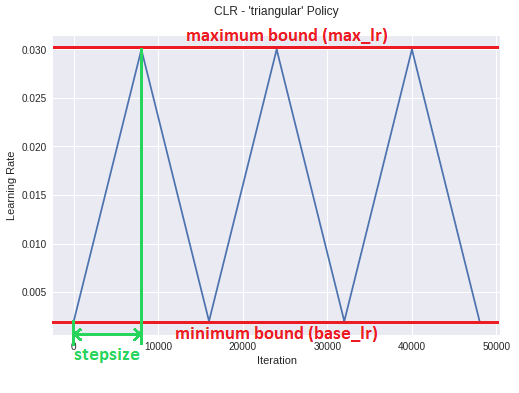
\includegraphics[width=0.45\textwidth]{images/it_lr_triangular.png} 
    \caption{Triangular learning rate policy. The blue lines represent learning rate values changing between red bounds. The input parameter step\_size is the number of iterations in half a cycle.}
    \label{fig:triang}
\end{figure}    
\begin{figure}[h!]
    \centering
    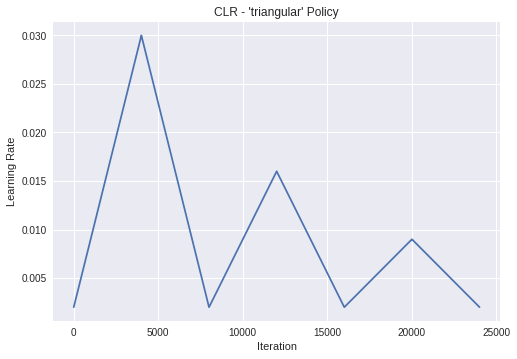
\includegraphics[width=0.45\textwidth]{images/it_lr_triang2.png} 
    \caption{Triangular 2 learning rate policy.}
    \label{fig:triang2}
\end{figure}    

\begin{figure}[h!]
    \centering
    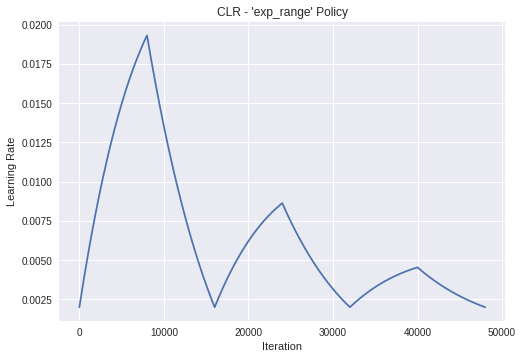
\includegraphics[width=0.45\textwidth]{images/it_lr_exp.png} 
    \caption{Exponential-range learning rate policy. }
    \label{fig:exp}
\end{figure}    
    Instead of using a fixed value for learning rate during the whole training process, it was shown in \cite{CLR} that oscillating the value inside a band helps to overpass saddle points plateaus more quickly.
    Updating the learning rate is done by using equations (1,2,3)\cite{CLR}.
    \begin{framed}
    \begin{eqnarray}
    lr = base\_lr + (max\_lr-base\_lr) * max(0,1-x)\\
    x = abs(iterations/step\_size - 2*cycle + 1)\\
    cycle = floor(1+iterations/(2*step\_size))
    \end{eqnarray}
    \end{framed}
    To dig a bit deeper, in Fig \ref{fig:triang}, $base\_lr$ and $max\_lr$ for the algorithm are initially tuned. Starting from iteration one, the learning rate starts with the base\_lr and moves towards the max\_lr in a defined manner which can be linear, exponential range or decaying triangular. Each step is defined to involve a number of iterations (or epochs) in a way that assures ending sharply at the end of a falling edge, i.e., steps number should be an even integer, see eq(7). The size of the data set considered for training should be dividable by the batch size to ensure safe termination. 
The method of cyclical learning rates consists of three different policies:
    \subsection{Triangular Policy}
    \label{sec:triang}
    This varies the learning rate linearly between the minimum ($base\_lr$) and the maximum ($max\_lr$) as shown in Figure \ref{fig:triang}.

    \subsection{Triangular 2 Policy}
    \label{sec:triang2}
    This policy is same as the triangular policy except that the maximum bound is cut in half at the end of each cycle as shown in Figure \ref{fig:triang2}. This means the learning rate difference decreases after each cycle and learning rate is defined as
    \begin{equation}
    \begin{split}
        lr = base\textunderscore lr + (max\_lr - base\_lr)*\\
    max(0, (1-x))/float(2^{cycle-1})
    \end{split}
    \end{equation}

    \subsection{Exponential range Policy}
    \label{sec:exp_range}
    This scales the cycle amplitude by a factor gamma (iterations), while keeping the $base\textunderscore lr$ constant as shown in Figure \ref{fig:exp}. The learning rate varies between the minimum and maximum boundaries and each boundary value declines by an exponential factor of gamma iteration and learning rate is calculated as
    \begin{equation}
    \begin{split}
lr=base\_lr + (max\_lr - base\_lr)* max(0,(1-x))\\
        *gamma^{iterations}            
    \end{split}
        \end{equation}

\section{Methodology}
\label{sec:methodology}
\subsection{CNN Architecture}
In this study we used Convolutional Neural Network (CNN) to test CLR approach. This architecture has 4 convolution layers, 2 max-pooling layers, 2 dropout layers and 3 fully connected layers with a final 2-way softmax activation, resulting in more than 225k parameters to be trained, Fig.\ref{fig:model_sum}.
Here we briefly discuss each layer. Fig. \ref{fig:architecture_cnn} shows the CNN architecture.
Each conv. layer has 32 neurons. Each neuron in the conv layers compute product between their weights and input volume that is connected to its local region and produce activation map. The weights and bias of the neuron are adjusted by training and CNN learn to respond to the activation. For faster training with gradient descent, Rectified Linear Unit(ReLu) is used.
The max pooling layers are used to reduce the spatial dimension of the input. We adopt pooling layers with filter of size 2 x 2 with a stride 2. In order to reduce test error and avoid over-fitting, dropout layer was implemented.
The layers fc1, fc2 and prediction shown in Fig are the fully-connected layers. Neuron in the fully connected layers have full connections to all neurons in the previous layer. The last layer of prediction consists of 2 neurons, and each score represents the confidence degree that the input belongs to positive or negative class.
	\begin{figure}[h!]
    \centering
    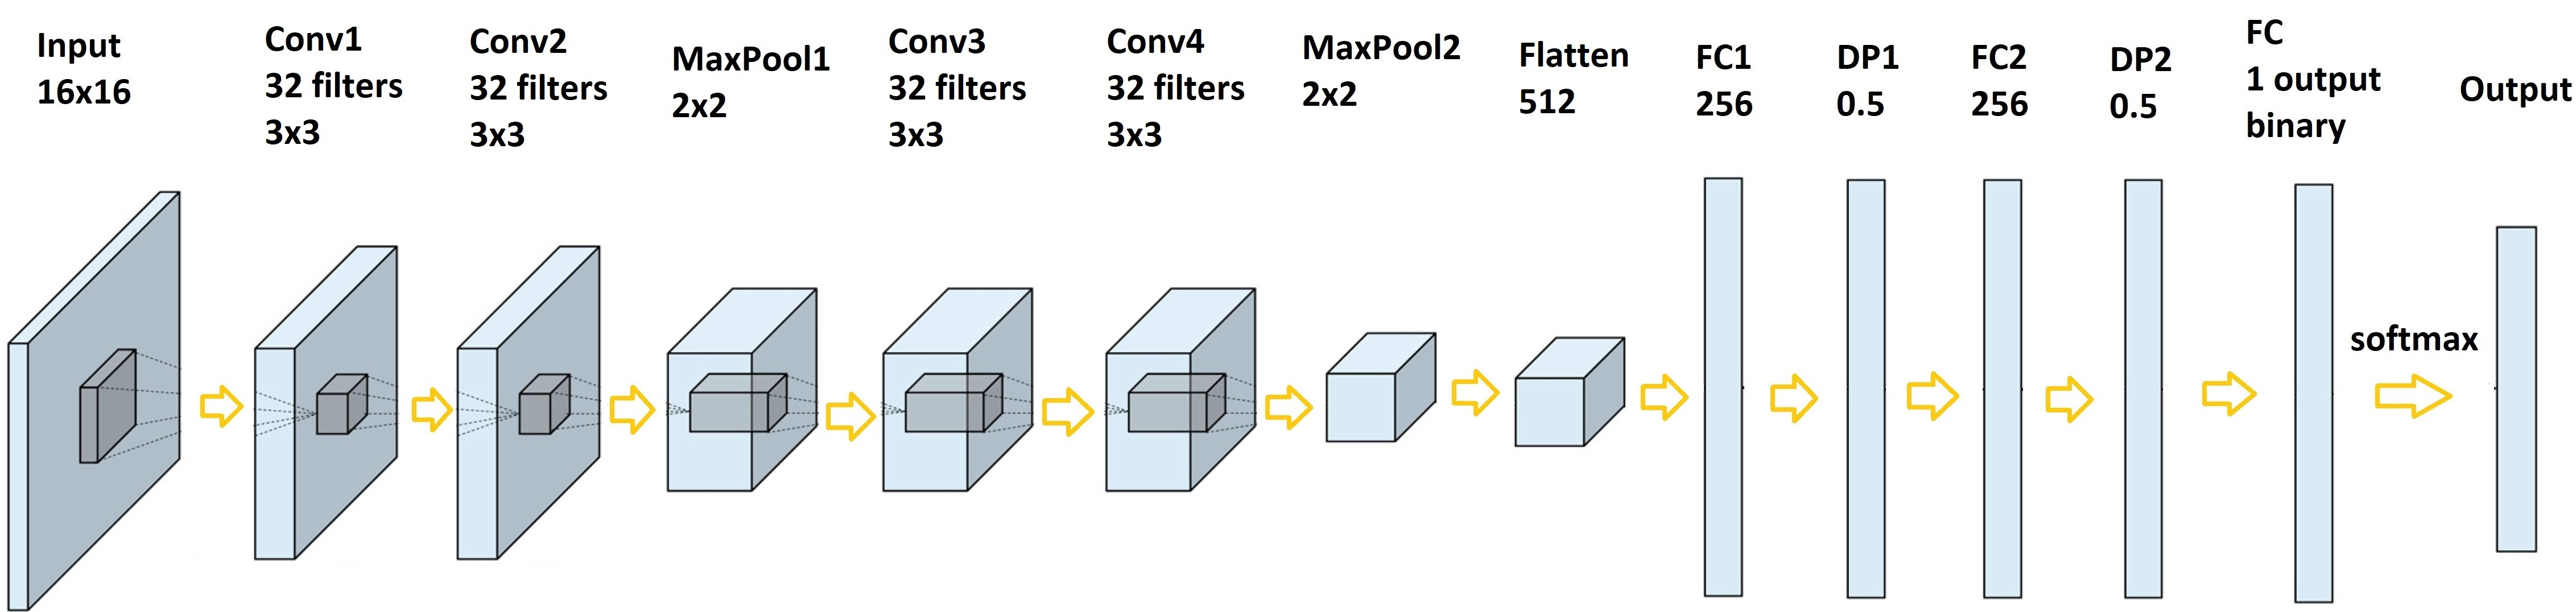
\includegraphics[width=0.45\textwidth]{images/architecture_cnn2.jpg} 
    \caption{CNN architecture}
    \label{fig:architecture_cnn}
    \end{figure}

    \begin{figure}[h!]
    \centering
    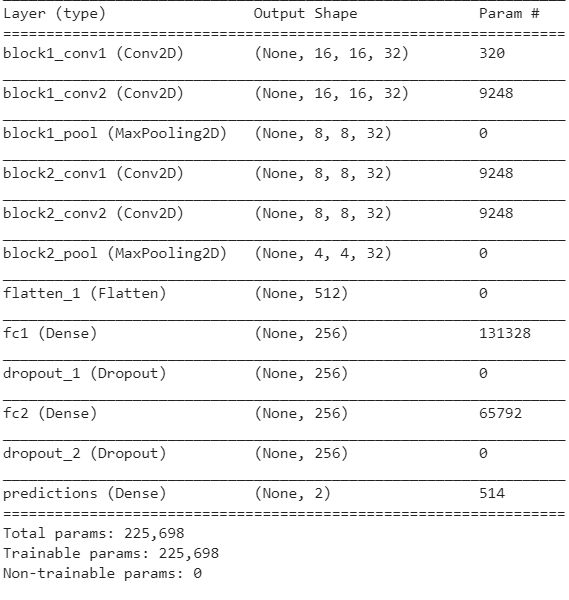
\includegraphics[width=0.45\textwidth]{images/parameters_achitec.png}
    \caption{Model summary}
    \label{fig:model_sum}
    \end{figure}
\subsection{Cycle Length Estimation}
In Cyclical learning rate, cycle length or step\_size (half of the cycle length) is an important parameter that affects results significantly. Authors in \cite{CLR} discuss the way of selecting the cycle length from the batch size and number of samples in the data set, eq (6). Step\_size can be calculated using the number of iteration per epoch. 
\begin{eqnarray}
iter\_per\_epoch = examples\_num / batchsize \\
steps\_num = num\_epochs / epochs\_per\_step
\end{eqnarray}
Authors suggested from their different experiments to set the step\_size 2 to 10 times of the number of iteration per epoch. Also, its better to end the training at the end of a cycle.
In our experiments we used two different conditions. In the first case 10 epochs were used with step\_size= 5*number of iteration per epoch, means half length of the circle is the 5 epoch and training ended at the end of the cycle. In the second case 12 epochs were used with $step\_size= 2 * iterations\_per\_epoch$ , means half length of the cycle is the 2 epoch and training was done by 3 complete cycles.

\subsection{Minimum and Maximum LR Boundary Estimation}
Another magnificent step in Cyclic learning rate is to estimate the base learning rate and maximum learning rate. Authors in \cite{CLR} proposed a simple approach of using “LR range test” by observing learning rate for a small number of epochs and observing the accuracy (with a balanced under-sampled data set).
Triangular policy can be used for LR range test. The testing was performed setting the lower bound to a small value (0.002), the max\_lr to 0.03 , and set the step\_size to the total number of iterations in the whole experiment ($epochs * iterations\_per\_epoch$) resulting in a linearly increasing learning rate, see Fig. \ref{fig:init_iter_lr}. After that, accuracy vs learning rate was plotted. Base learning should be the point from where accuracy starts increasing and max learning rate to be the learning rate where accuracy starts to slow down, oscillate, or fall \cite{CLR}. Fig. \ref{fig:init_lr_acc} was analyzed, base\_lr selected to be 0.002 and max\_lr to be 0.03.
As the data set used in our experiments was highly unbalanced, accuracy was not a good performance measure. In our LR test, balanced subset of the entire data set was used consisting 6000 samples 3000 for each class.
    \begin{figure}[h!]
    \centering
    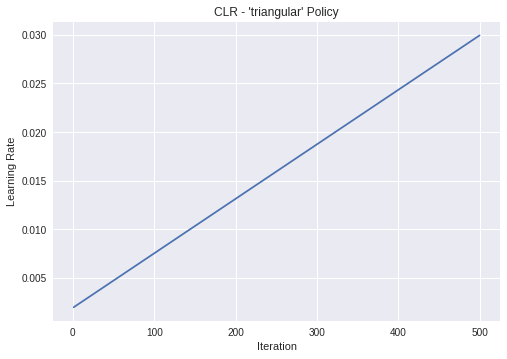
\includegraphics[width=0.45\textwidth]{images/init_iter_vs_lr.png} 
    \caption{Initialization, iteration vs learning rate}
    \label{fig:init_iter_lr}
    \end{figure}

    \begin{figure}[h!]
    \centering
    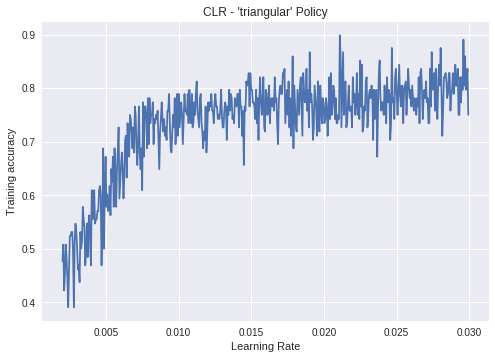
\includegraphics[width=0.45\textwidth]{images/init_lr_vs_accuracy.png}
    \caption{Initialization, learning rate vs accuracy}
    \label{fig:init_lr_acc}
    \end{figure}

\section{Environment and Experiments }
\subsection{Environment}
	All experiments were carried out using \textsc{Google Colaboratory} web service. \textsc{Colaboratory} is a Google research project created to help disseminate machine learning education and research. It is a  helpful and free cloud service which can be used to develop deep learning applications using Python. It is a Jupyter notebook that requires no installation to use and runs entirely on the cloud. The implementation of neural network was carried out using the sequential model of Keras \cite{keras}. All measurements were made using \textsc{sklearn} \cite{sklearn}, while ROC and Precision-Recall plots were made using \textsc{Scikit-plot} \cite{scikitplot}
	
	\begin{table}[hbt]
		% Center the table
		\begin{center}
		% Title of the table
		\caption{Environment Properties}
		\label{tab:simParameters}
		% Table itself: here we have two columns which are centered and have lines to the left, right and in the middle: |c|c|
		\begin{tabular}{|c|c|}
			% To create a horizontal line, type \hline
			\hline
			% To end a column type &
			% For a linebreak type \\
			PROPERTY & VALUE \\
			\hline
			CPU & Intel® Xeon® CPU @ 2.20GHz, 1 core \\
			\hline
			RAM & 12GB\\
			\hline
			GPU & Nvidia Tesla K80, 24GB\\
			\hline
		\end{tabular}
		\end{center}
	\end{table}	
\subsection{Experiments}
Two values of skewness were used to reflect realistic results. With the first case, skewness = 1/17, i.e., for each positive example there exist 17 different negative examples. To visualize the performance of the classifier, ROC and Precision-Recall curves were used along with the area under them. Accuracy could have been a misleading choice if it had been used with imbalanced data sets. In the second case, skewness was set to 1/36. For hyper-parameters values, see TABLE \ref{tab:hyper_val}.
For every case, three runs were averaged to check the stability of results with different random initializations.

\subsection{Case 1, Skewness = 1/17}
Table \ref{tab:sk17mean} show the average results for triangular, triangular2, exp\_range and fixed. From the table, it is clear that exp\_range is relatively better among others with high F1 score and AUC with small deviations.
All policies outperformed the fixed learning rate with lr = 0.002 (base\_lr).
\begin{table}[h]
    \centering
    \begin{tabular}{c|c|c}
        \textbf{\uppercase {Hyp-Param}} & \textbf{\uppercase{Value}} \\ \hline
        epochs              &  12                     \\ \hline
        basel\_lr           &   0.002                          \\ \hline
        max\_lr             &  0.03     \\ \hline
        batch\_size         & 32                \\ \hline
        Train set size      &64k (case 1), 128k( case 2)                 \\ \hline
        epochs per step     &  2              \\ \hline
    \end{tabular}
    \caption{Hyper-parameters values}
    \label{tab:hyper_val}
\end{table}
\import{tables/}{sk17mean.tex}
\import{tables/}{sk17std.tex}
\subsection{Case 2, Skewness = 1/36}
TABLE \ref{tab:sk36mean} and TABLE \ref{tab:sk36std} show results for the second case.
Here, the fixed policy gave the worst results among others, it gave around AUC = 0.38 with very low precision recall with learning rate = 0.002. While triangular1 and triangular2 are best performing. Fig \ref{fig:triang1_roc_test} and Fig. \ref{fig:triang1_pr_test} show ROC and precision-recall curves, respectively.

\import{tables/}{sk36mean.tex}
\import{tables/}{sk36std.tex}
\begin{figure}[h]
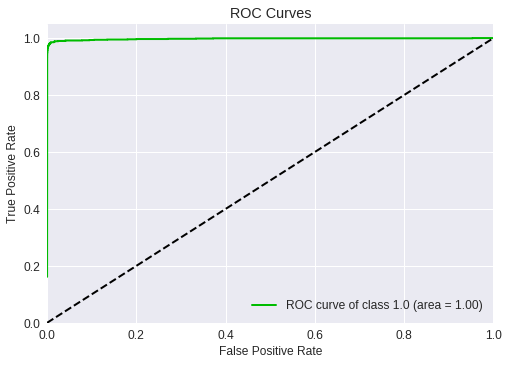
\includegraphics[scale=0.45]{images/skew36/triangular1/roc_triang_test.png}
\caption{ROC curve for triangular 1, skew = 1/36}
\label{fig:triang1_roc_test}
\end{figure}
\begin{figure}[h!]
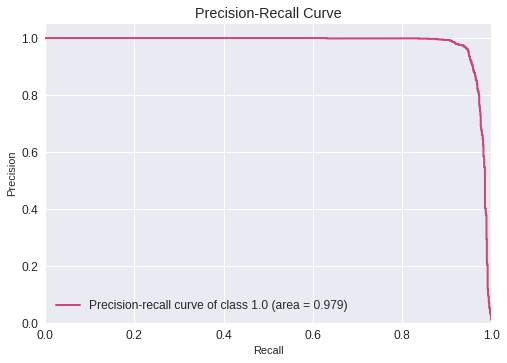
\includegraphics[scale=0.45]{images/skew36/triangular1/PR_triang_test.png}
\caption{PR curve for triangular 1, skew = 1/36}
\label{fig:triang1_pr_test}
\end{figure}
\section{Conclusion}
The experimental results presented in this paper demonstrate the benefits of using cyclical learning rate (CLR) method for unbalanced data sets. These cyclical variations for the learning rate between the base\_lr and max\_lr can provide optimal classification results, also in case of highly-skewed unbalanced data sets. Simple LR range test can provide the estimation of the learning rate boundaries avoiding the computational complexity and expense of tuning the classifier model with fixed learning rate. We tried different modes of triangular learning rate with a simple CNN with a few epochs to train and test on unbalanced data set. In comparison with fixed learning rate, all the cases of CLR provided better metrics (AUC, and F1 score). In future Clr could be applied on deeper CNN with different architectures to check its performance.
% Now we need a bibliography:
\begin{thebibliography}{5}
    
	%Each item starts with a \bibitem{reference} command and the details thereafter.
	\bibitem{CLR}
	Leslie~N.~Smith. Cyclical Learning Rates for Training Neural Networks. {\em CoRR},
	U.S. Naval Research Laboratory, \url{http://arxiv.org/abs/1506.01186}, Apr. 2017.
    
    \bibitem{keras}
	Chollet, Fran\c{c}ois and others. Keras. \url{https://keras.io},
    2015.

    \bibitem{sklearn}
	Pedregosa,~F. and Varoquaux,~G. and Gramfort,~A. and Michel,~V.
    and Thirion,~B. and Grisel,~O. and Blondel,~M. and Prettenhofer,~P.
    and Weiss,~R. and Dubourg,~V. and Vanderplas,~J. and Passos,~A. and
    Cournapeau,~D. and Brucher,~M. and Perrot,~M. and Duchesnay,~E. Scikit-learn: Machine Learning in {P}ython. {\em Journal of Machine Learning Research},
	vol.~12, pp.~2825--2830, 2011.
	
	\bibitem{scikitplot}
	Reiichiro Nakano. (2017, February 19). reiinakano/scikit-plot: v0.2.1 (Version v0.2.1). Zenodo. http://doi.org/10.5281/zenodo.293191.
	
\end{thebibliography}

% Your document ends here!
\end{document}